\section{Behavioral Design}
\label{sec:sd-behavior}

\subsection{Run Lifecycle}
\label{sec:sd-run-lifecycle}

Work starts from the chat box: creating a thread starts nothing, the first message does. The first run of a project begins at the planner, and every later run, in any thread of the project, begins at the intent router (Figure~\ref{fig:sd-run-entry}).

\begin{figure}[H]
    \centering
    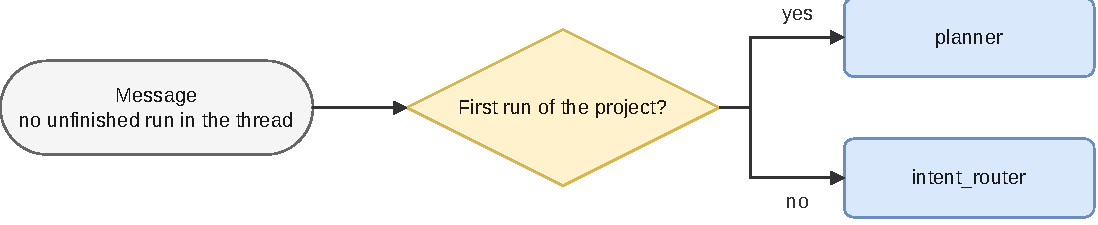
\includegraphics[width=0.75\linewidth]{system-design/runtime-run-entry.pdf}
    \caption{Where a run begins in the workflow.}
    \label{fig:sd-run-entry}
\end{figure}

A run is a resource with a lifecycle (Figure~\ref{fig:sd-run-lifecycle}). It is \emph{unfinished} while it is \texttt{queued}, \texttt{running} or \texttt{interrupted}, and \emph{finished} once it is \texttt{succeeded}, \texttt{failed} or \texttt{cancelled}; a finished run never changes status again. An interrupted run waits for the user at a checkpoint with no time limit. A thread has at most one unfinished run.

\begin{figure}[H]
    \centering
    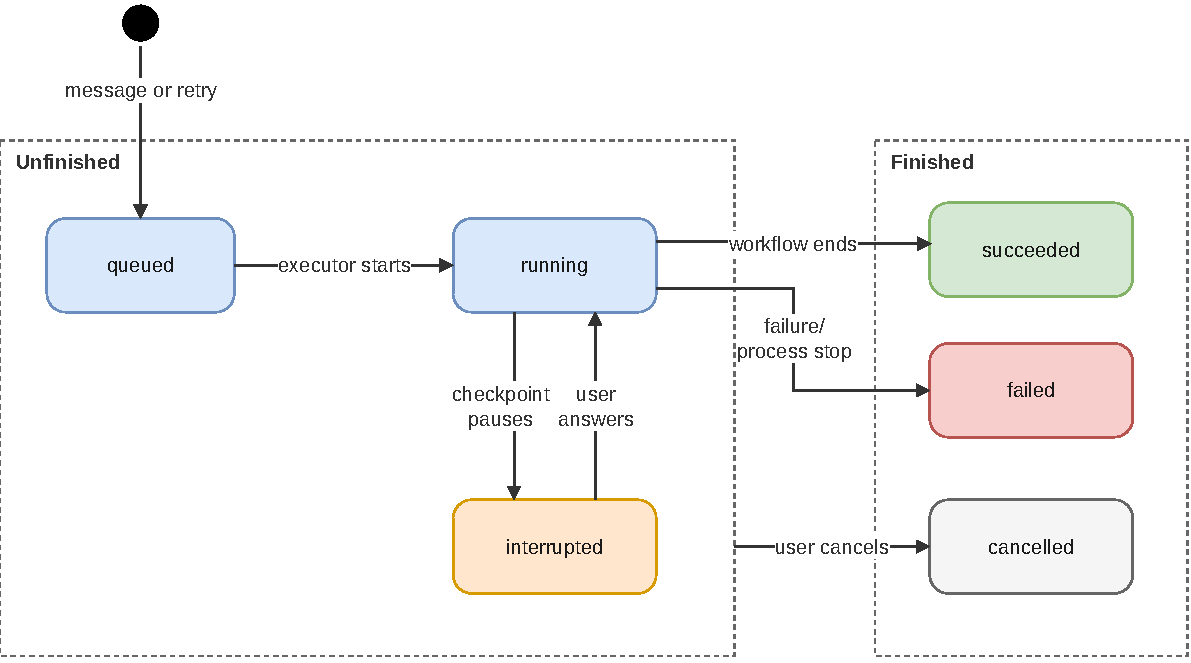
\includegraphics[width=0.7\linewidth]{system-design/runtime-run-lifecycle.pdf}
    \caption{State diagram of a run.}
    \label{fig:sd-run-lifecycle}
\end{figure}

\subsection{Steps of a Node}
\label{sec:sd-node-steps}

Figure~\ref{fig:sd-node-steps} shows what happens at every node of a run. Before a node calls an LLM, the cost limit of the run and the budget of the user are checked, so that a run fails before it overspends rather than after. The node then calls the model, writes its items through the integrity checks, and appends its events to the event log. At a checkpoint node the run is interrupted until the user chooses an option. After each node the state is saved: this \emph{safe point} is where a failed run can be retried from, and where pending user messages are taken in by the intent router.

\begin{figure}[H]
    \centering
    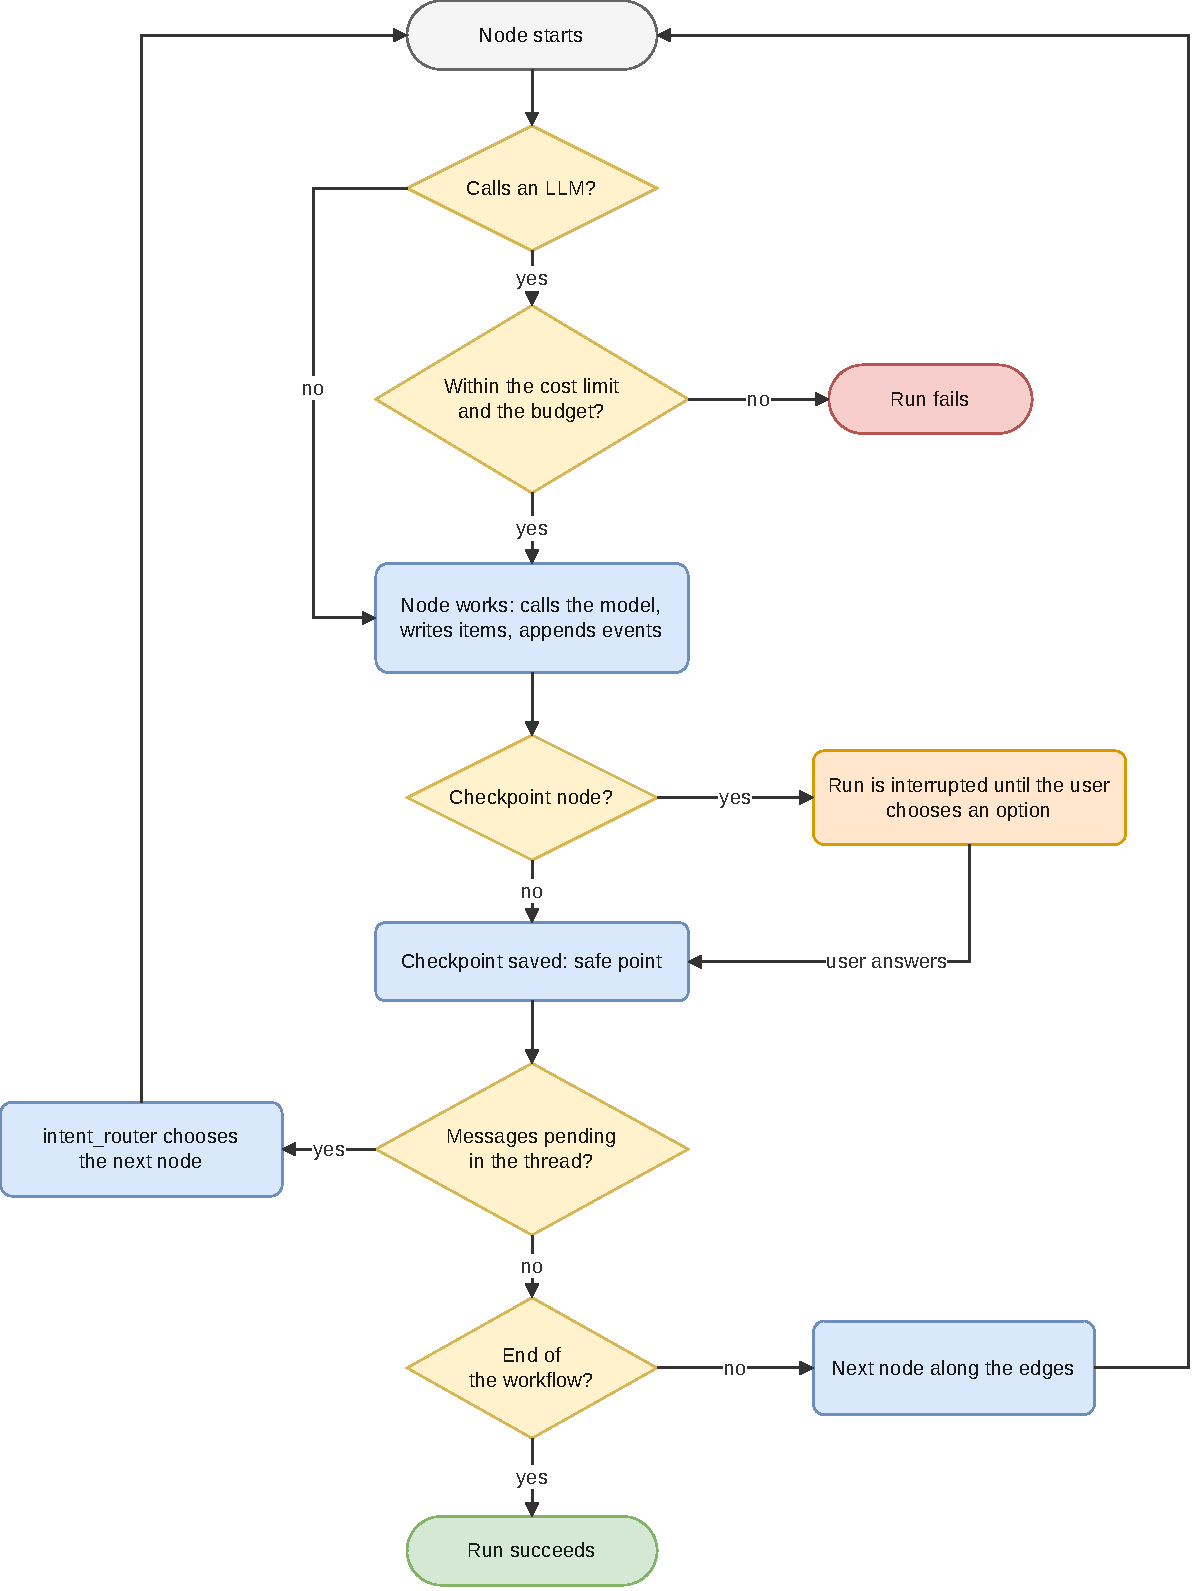
\includegraphics[height=0.62\textheight]{system-design/runtime-node-steps.pdf}
    \caption{Activity diagram of one node of a run.}
    \label{fig:sd-node-steps}
\end{figure}

\subsection{Messages During a Run}
\label{sec:sd-messages}

A message the user sends while a run is unfinished is stored as \emph{pending}. It becomes \emph{delivered} when the intent router takes it in at the next safe point, and \emph{undelivered} if the run fails or is cancelled first, in which case the user can send it again (Figure~\ref{fig:sd-message-delivery}). A message sent when no run is unfinished starts a new run.

\begin{figure}[H]
    \centering
    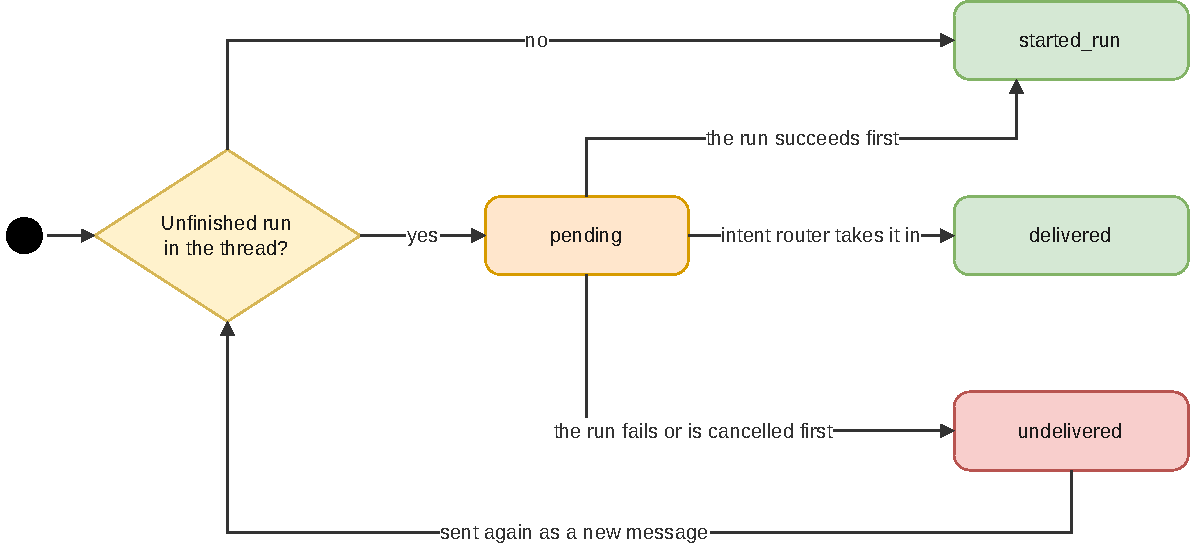
\includegraphics[width=0.75\linewidth]{system-design/runtime-message-delivery.pdf}
    \caption{State diagram of a user message.}
    \label{fig:sd-message-delivery}
\end{figure}

\subsection{Sequence of a Run}
\label{sec:sd-sequence}

Figure~\ref{fig:sd-sequence} shows the interactions of use case UC-01 and UC-02. The essential property is that the workflow never writes into an HTTP response: it appends events to the event log in the database, and the stream endpoint reads the log. The request that starts a run therefore returns at once, a closed browser does not stop the run, and a client that reconnects receives the events it missed by sending the identifier of the last event it saw.

\begin{figure}[H]
    \centering
    \resizebox{\linewidth}{!}{%
    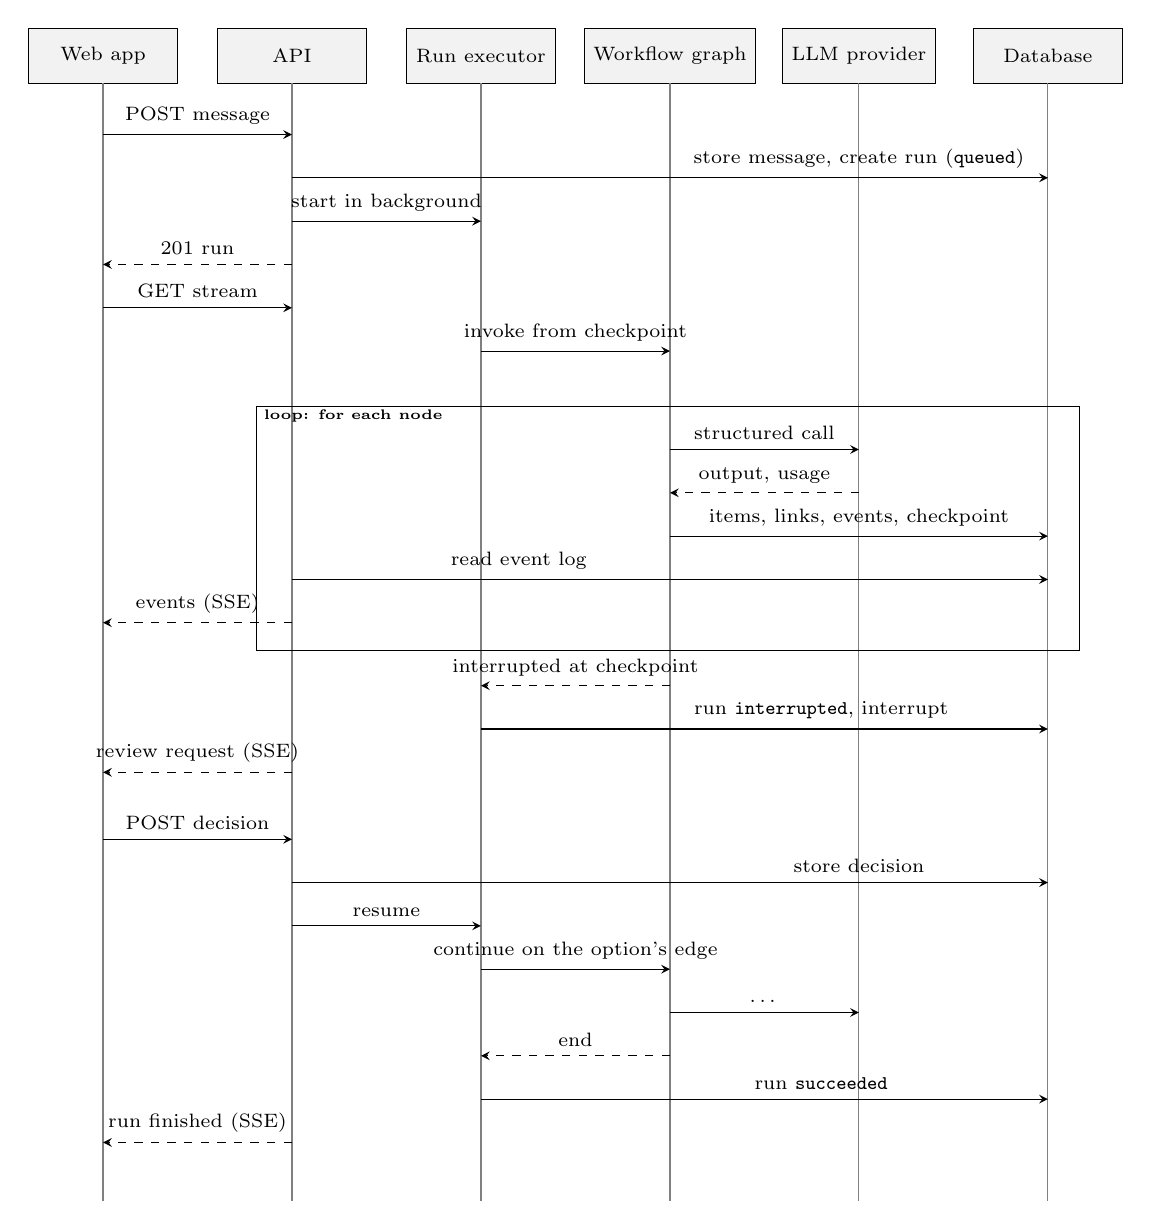
\begin{tikzpicture}[
        font=\scriptsize,
        life/.style={draw, fill=gray!10, minimum width=1.9cm, minimum height=0.7cm, align=center},
        msg/.style={->, >=stealth},
        ret/.style={->, >=stealth, dashed}
    ]
        \foreach \name/\label/\x in {web/Web app/0, api/API/2.4, exe/Run executor/4.8, graph/Workflow graph/7.2, llm/LLM provider/9.6, db/Database/12.0} {
            \node[life] (\name) at (\x, 0) {\label};
            \draw[gray] (\x, -0.35) -- (\x, -14.55);
        }
        \draw[msg] (0,-1.00) -- node[above] {POST message} (2.4,-1.00);
        \draw[msg] (2.4,-1.55) -- node[above, pos=0.75] {store message, create run (\texttt{queued})} (12.0,-1.55);
        \draw[msg] (2.4,-2.10) -- node[above] {start in background} (4.8,-2.10);
        \draw[ret] (2.4,-2.65) -- node[above] {201 run} (0,-2.65);
        \draw[msg] (0,-3.20) -- node[above] {GET stream} (2.4,-3.20);
        \draw[msg] (4.8,-3.75) -- node[above] {invoke from checkpoint} (7.2,-3.75);
        \node[font=\tiny\bfseries, anchor=north west, inner sep=1pt] at (2.0,-4.45) {loop: for each node};
        \draw[msg] (7.2,-5.00) -- node[above] {structured call} (9.6,-5.00);
        \draw[ret] (9.6,-5.55) -- node[above] {output, usage} (7.2,-5.55);
        \draw[msg] (7.2,-6.10) -- node[above] {items, links, events, checkpoint} (12.0,-6.10);
        \draw[msg] (2.4,-6.65) -- node[above, pos=0.3] {read event log} (12.0,-6.65);
        \draw[ret] (2.4,-7.20) -- node[above] {events (SSE)} (0,-7.20);
        \draw (1.95,-4.45) rectangle (12.4,-7.55);
        \draw[ret] (7.2,-8.00) -- node[above] {interrupted at checkpoint} (4.8,-8.00);
        \draw[msg] (4.8,-8.55) -- node[above, pos=0.6] {run \texttt{interrupted}, interrupt} (12.0,-8.55);
        \draw[ret] (2.4,-9.10) -- node[above] {review request (SSE)} (0,-9.10);
        \draw[msg] (0,-9.95) -- node[above] {POST decision} (2.4,-9.95);
        \draw[msg] (2.4,-10.50) -- node[above, pos=0.75] {store decision} (12.0,-10.50);
        \draw[msg] (2.4,-11.05) -- node[above] {resume} (4.8,-11.05);
        \draw[msg] (4.8,-11.60) -- node[above] {continue on the option's edge} (7.2,-11.60);
        \draw[msg] (7.2,-12.15) -- node[above] {\ldots} (9.6,-12.15);
        \draw[ret] (7.2,-12.70) -- node[above] {end} (4.8,-12.70);
        \draw[msg] (4.8,-13.25) -- node[above, pos=0.6] {run \texttt{succeeded}} (12.0,-13.25);
        \draw[ret] (2.4,-13.80) -- node[above] {run finished (SSE)} (0,-13.80);
    \end{tikzpicture}}
    \caption{Sequence diagram of starting a run and answering a checkpoint (UC-01 and UC-02).}
    \label{fig:sd-sequence}
\end{figure}

\subsection{Failures, Cancellation and Restarts}
\label{sec:sd-failures}

A step that fails, for example because a provider returns an error or an agent output fails the integrity checks, ends the run as \texttt{failed} with an error code. The user can retry it: the retry starts a new run from the last completed step, using the saved checkpoint, so the LLM calls of earlier steps are not made again. Cancellation stops the run at the next safe point. Since runs execute as tasks inside the API process, a restart of the process ends the steps in progress: on startup the API marks those runs as \texttt{failed} with the code \texttt{server\_restarted}, starts again the runs that were still \texttt{queued}, and leaves interrupted runs waiting for the user.
